\documentclass[11pt]{article}
\usepackage{tikz}
\usepackage{amssymb}
\usepackage{geometry}
\geometry{letterpaper, landscape, margin=0.4in}
\usetikzlibrary{positioning, calc}

% Door macros
\newcommand{\hdoor}[2]{%
  \fill[white,draw=black,thick] ({#1-0.1},{#2-0.12}) rectangle ({#1+0.1},{#2+0.12});%
}
\newcommand{\vdoor}[2]{%
  \fill[white,draw=black,thick] ({#1-0.12},{#2-0.1}) rectangle ({#1+0.12},{#2+0.1});%
}

\begin{document}

\begin{center}
{\Huge \textbf{THE GRAIN MOTHER'S RUIN}}\\[0.3em]
{\Large Level 2 --- The Vaults Below | 25 Keyed Areas}
\end{center}

\vspace{0.3em}

\begin{center}
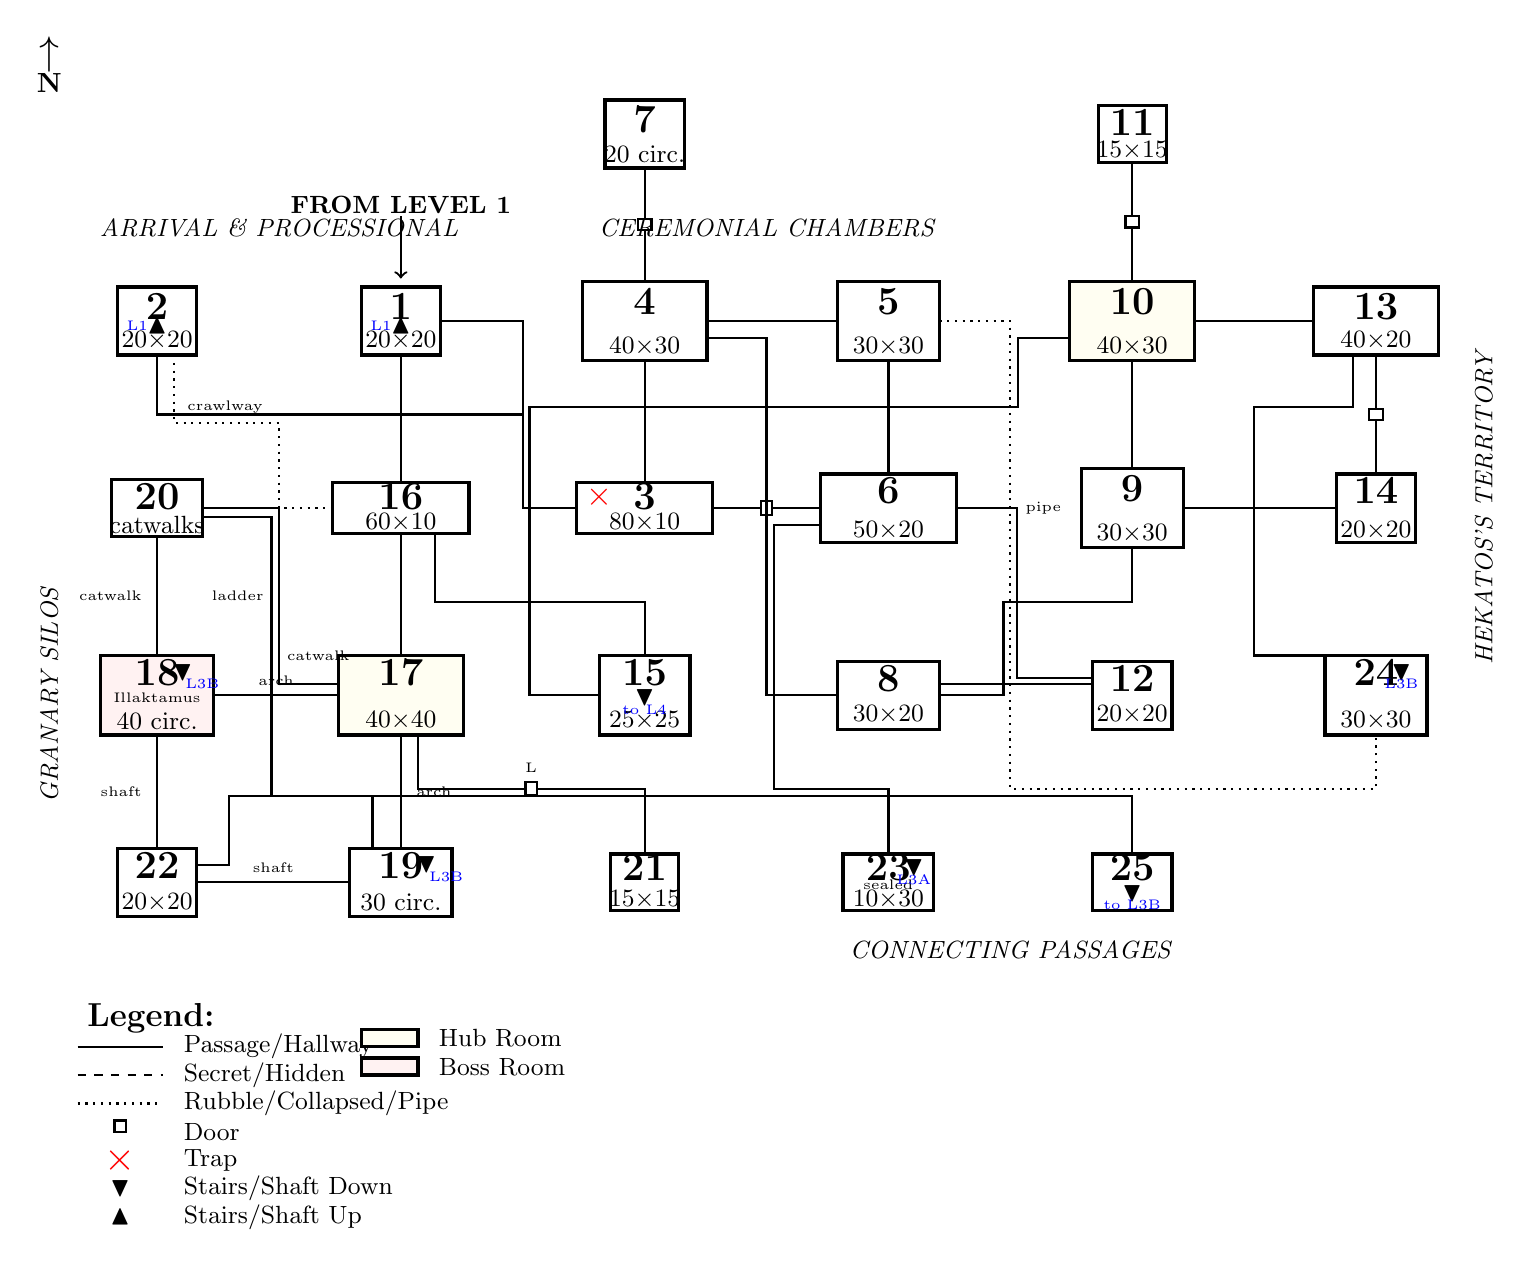
\begin{tikzpicture}[
    room/.style={draw, very thick, rectangle},
    hub/.style={draw, very thick, rectangle, fill=yellow!5},
    boss/.style={draw, very thick, rectangle, fill=red!5},
    connection/.style={draw, thick},
    secret/.style={dashed, thick},
    trap/.style={red},
    scale=0.72
]

% ============================================================
% Grid: 6 cols x 5 rows | CellW=2.8, CellH=1.8, Gutter=1.5
% Col centers: c0=1.4, c1=5.7, c2=10.0, c3=14.3, c4=18.6, c5=22.9
% Row centers: r0=0.9, r1=4.2, r2=7.5, r3=10.8, r4=14.1
% Vert gutters: g01=3.55, g12=7.85, g23=12.15, g34=16.45, g45=20.75
% Horiz gutters: g01=2.55, g12=5.85, g23=9.15, g34=12.45
% Room rect max: 2.4 wide x 1.5 tall (min 1.2 x 0.8)
% ============================================================

% ============================================================
% NORTH ARROW
% ============================================================
\node at (-0.5,15.5) {\Large $\uparrow$};
\node at (-0.5,15.0) {\textbf{N}};

% ENTRANCE label (Room 1 stairs from Level 1)
\node[font=\small\bfseries] at (5.7,12.85) {FROM LEVEL 1};
\draw[->, thick] (5.7,12.65) -- (5.7,11.55);

% ============================================================
% ZONE: ARRIVAL & PROCESSIONAL (Rooms 1--3)
% Grid region: cols 1--2, rows 2--3
% ============================================================

% Room 1: The Stair Landing (20x20 ft)
% Cell: (1,3) -> center (5.7, 10.8)
% Rect: 1.4w x 1.2h -> (5.0, 10.2) to (6.4, 11.4)
\draw[room] (5.0,10.2) rectangle (6.4,11.4);
\node at (5.7,11.05) {\Large \textbf{1}};
\node[font=\small] at (5.7,10.45) {20$\times$20};
\node at (5.7,10.72) {$\blacktriangle$};
\node[font=\tiny,blue] at (5.35,10.72) {L1};

% Room 2: The Collapsed Shaft (20 irreg.)
% Cell: (0,3) -> center (1.4, 10.8)
% Rect: 1.4w x 1.2h -> (0.7, 10.2) to (2.1, 11.4)
\draw[room] (0.7,10.2) rectangle (2.1,11.4);
\node at (1.4,11.05) {\Large \textbf{2}};
\node[font=\small] at (1.4,10.45) {20$\times$20};
\node at (1.4,10.72) {$\blacktriangle$};
\node[font=\tiny,blue] at (1.05,10.72) {L1};

% Room 3: The Processional Corridor (80x10 ft)
% Cell: (2,2) -> center (10.0, 7.5)
% Rect: 2.4w x 0.9h -> (8.8, 7.05) to (11.2, 7.95)
\draw[room] (8.8,7.05) rectangle (11.2,7.95);
\node at (10.0,7.7) {\Large \textbf{3}};
\node[font=\small] at (10.0,7.25) {80$\times$10};
% Trap marker (pressure plate at midpoint)
\node[red] at (9.2,7.7) {\large $\times$};

% ============================================================
% ZONE: CEREMONIAL CHAMBERS (Rooms 4--7)
% Grid region: cols 2--3, rows 2--4
% ============================================================

% Room 4: The Robing Hall (40x30 ft)
% Cell: (2,3) -> center (10.0, 10.8)
% Rect: 2.2w x 1.4h -> (8.9, 10.1) to (11.1, 11.5)
\draw[room] (8.9,10.1) rectangle (11.1,11.5);
\node at (10.0,11.15) {\Large \textbf{4}};
\node[font=\small] at (10.0,10.35) {40$\times$30};

% Room 5: The Purification Baths (30x30 ft)
% Cell: (3,3) -> center (14.3, 10.8)
% Rect: 1.8w x 1.4h -> (13.4, 10.1) to (15.2, 11.5)
\draw[room] (13.4,10.1) rectangle (15.2,11.5);
\node at (14.3,11.15) {\Large \textbf{5}};
\node[font=\small] at (14.3,10.35) {30$\times$30};

% Room 6: The Hall of Inscriptions (50x20 ft)
% Cell: (3,2) -> center (14.3, 7.5)
% Rect: 2.4w x 1.2h -> (13.1, 6.9) to (15.5, 8.1)
\draw[room] (13.1,6.9) rectangle (15.5,8.1);
\node at (14.3,7.8) {\Large \textbf{6}};
\node[font=\small] at (14.3,7.1) {50$\times$20};

% Room 7: The Vigil Chamber (20 diam circular)
% Cell: (2,4) -> center (10.0, 14.1)
% Rect: 1.4w x 1.2h -> (9.3, 13.5) to (10.7, 14.7)
\draw[room] (9.3,13.5) rectangle (10.7,14.7);
\node at (10.0,14.35) {\Large \textbf{7}};
\node[font=\small] at (10.0,13.75) {20 circ.};

% ============================================================
% ZONE: HEKATOS'S TERRITORY (Rooms 8--15)
% Grid region: cols 3--5, rows 1--4
% ============================================================

% Room 8: The Outer Ward (30x20 ft)
% Cell: (3,1) -> center (14.3, 4.2)
% Rect: 1.8w x 1.2h -> (13.4, 3.6) to (15.2, 4.8)
\draw[room] (13.4,3.6) rectangle (15.2,4.8);
\node at (14.3,4.5) {\Large \textbf{8}};
\node[font=\small] at (14.3,3.85) {30$\times$20};

% Room 9: The Disciple Quarters (30x30 ft)
% Cell: (4,2) -> center (18.6, 7.5)
% Rect: 1.8w x 1.4h -> (17.7, 6.8) to (19.5, 8.2)
\draw[room] (17.7,6.8) rectangle (19.5,8.2);
\node at (18.6,7.85) {\Large \textbf{9}};
\node[font=\small] at (18.6,7.05) {30$\times$30};

% Room 10: The Research Chamber (40x30 ft) -- HUB
% Cell: (4,3) -> center (18.6, 10.8)
% Rect: 2.2w x 1.4h -> (17.5, 10.1) to (19.7, 11.5)
\draw[hub] (17.5,10.1) rectangle (19.7,11.5);
\node at (18.6,11.15) {\Large \textbf{10}};
\node[font=\small] at (18.6,10.35) {40$\times$30};

% Room 11: Hekatos's Private Study (15x15 ft)
% Cell: (4,4) -> center (18.6, 14.1)
% Rect: 1.2w x 1.0h -> (18.0, 13.6) to (19.2, 14.6)
\draw[room] (18.0,13.6) rectangle (19.2,14.6);
\node at (18.6,14.3) {\Large \textbf{11}};
\node[font=\small] at (18.6,13.8) {15$\times$15};

% Room 12: The Ward-Stone Chamber (20x20 ft)
% Cell: (4,1) -> center (18.6, 4.2)
% Rect: 1.4w x 1.2h -> (17.9, 3.6) to (19.3, 4.8)
\draw[room] (17.9,3.6) rectangle (19.3,4.8);
\node at (18.6,4.5) {\Large \textbf{12}};
\node[font=\small] at (18.6,3.85) {20$\times$20};

% Room 13: The Archives (40x20 ft)
% Cell: (5,3) -> center (22.9, 10.8)
% Rect: 2.2w x 1.2h -> (21.8, 10.2) to (24.0, 11.4)
\draw[room] (21.8,10.2) rectangle (24.0,11.4);
\node at (22.9,11.05) {\Large \textbf{13}};
\node[font=\small] at (22.9,10.45) {40$\times$20};

% Room 14: The Alchemical Workshop (20x20 ft)
% Cell: (5,2) -> center (22.9, 7.5)
% Rect: 1.4w x 1.2h -> (22.2, 6.9) to (23.6, 8.1)
\draw[room] (22.2,6.9) rectangle (23.6,8.1);
\node at (22.9,7.8) {\Large \textbf{14}};
\node[font=\small] at (22.9,7.1) {20$\times$20};

% Room 15: The Sealed Descent (25x25 ft)
% Cell: (2,1) -> center (10.0, 4.2)
% Rect: 1.6w x 1.4h -> (9.2, 3.5) to (10.8, 4.9)
\draw[room] (9.2,3.5) rectangle (10.8,4.9);
\node at (10.0,4.6) {\Large \textbf{15}};
\node[font=\small] at (10.0,3.75) {25$\times$25};
\node at (10.0,4.15) {$\blacktriangledown$};
\node[font=\tiny,blue] at (10.0,3.95) {to L4};

% ============================================================
% ZONE: GRANARY SILOS (Rooms 16--22)
% Grid region: cols 0--1, rows 0--2
% ============================================================

% Room 16: The Silo Approach (60x10 ft)
% Cell: (1,2) -> center (5.7, 7.5)
% Rect: 2.4w x 0.9h -> (4.5, 7.05) to (6.9, 7.95)
\draw[room] (4.5,7.05) rectangle (6.9,7.95);
\node at (5.7,7.7) {\Large \textbf{16}};
\node[font=\small] at (5.7,7.25) {60$\times$10};

% Room 17: The Loading Hall (40x40 ft) -- HUB (silo hub)
% Cell: (1,1) -> center (5.7, 4.2)
% Rect: 2.2w x 1.4h -> (4.6, 3.5) to (6.8, 4.9)
\draw[hub] (4.6,3.5) rectangle (6.8,4.9);
\node at (5.7,4.6) {\Large \textbf{17}};
\node[font=\small] at (5.7,3.75) {40$\times$40};

% Room 18: Upper Silo West -- Illaktamus's Lair (40 diam) -- BOSS
% Cell: (0,1) -> center (1.4, 4.2)
% Rect: 2.0w x 1.4h -> (0.4, 3.5) to (2.4, 4.9)
\draw[boss] (0.4,3.5) rectangle (2.4,4.9);
\node at (1.4,4.6) {\Large \textbf{18}};
\node[font=\small] at (1.4,3.75) {40 circ.};
\node[font=\tiny] at (1.4,4.15) {Illaktamus};
\node at (1.85,4.6) {$\blacktriangledown$};
\node[font=\tiny,blue] at (2.2,4.4) {L3B};

% Room 19: Upper Silo East (30 diam)
% Cell: (1,0) -> center (5.7, 0.9)
% Rect: 1.8w x 1.2h -> (4.8, 0.3) to (6.6, 1.5)
\draw[room] (4.8,0.3) rectangle (6.6,1.5);
\node at (5.7,1.2) {\Large \textbf{19}};
\node[font=\small] at (5.7,0.55) {30 circ.};
\node at (6.15,1.2) {$\blacktriangledown$};
\node[font=\tiny,blue] at (6.5,1.0) {L3B};

% Room 20: The Silo Catwalks (walkways)
% Cell: (0,2) -> center (1.4, 7.5)
% Rect: 1.6w x 1.0h -> (0.6, 7.0) to (2.2, 8.0)
\draw[room] (0.6,7.0) rectangle (2.2,8.0);
\node at (1.4,7.7) {\Large \textbf{20}};
\node[font=\small] at (1.4,7.2) {catwalks};

% Room 21: The Grain-Master's Vault (15x15 ft)
% Cell: (2,0) -> center (10.0, 0.9)
% Rect: 1.2w x 1.0h -> (9.4, 0.4) to (10.6, 1.4)
\draw[room] (9.4,0.4) rectangle (10.6,1.4);
\node at (10.0,1.15) {\Large \textbf{21}};
\node[font=\small] at (10.0,0.6) {15$\times$15};

% Room 22: The Silo Floor Access (20x20 ft)
% Cell: (0,0) -> center (1.4, 0.9)
% Rect: 1.4w x 1.2h -> (0.7, 0.3) to (2.1, 1.5)
\draw[room] (0.7,0.3) rectangle (2.1,1.5);
\node at (1.4,1.2) {\Large \textbf{22}};
\node[font=\small] at (1.4,0.55) {20$\times$20};

% ============================================================
% ZONE: CONNECTING PASSAGES (Rooms 23--25)
% Grid region: cols 3--4, row 0
% ============================================================

% Room 23: The Sealed Passage (10x30 ft)
% Cell: (3,0) -> center (14.3, 0.9)
% Rect: 1.6w x 1.0h -> (13.5, 0.4) to (15.1, 1.4)
\draw[room] (13.5,0.4) rectangle (15.1,1.4);
\node at (14.3,1.15) {\Large \textbf{23}};
\node[font=\small] at (14.3,0.6) {10$\times$30};
\node[font=\tiny] at (14.3,0.85) {sealed};
\node at (14.75,1.15) {$\blacktriangledown$};
\node[font=\tiny,blue] at (14.75,0.95) {L3A};

% Room 24: The Flooded Cistern (30x30 ft)
% Cell: (5,1) -> center (22.9, 4.2)
% Rect: 1.8w x 1.4h -> (22.0, 3.5) to (23.8, 4.9)
\draw[room] (22.0,3.5) rectangle (23.8,4.9);
\node at (22.9,4.6) {\Large \textbf{24}};
\node[font=\small] at (22.9,3.75) {30$\times$30};
\node at (23.35,4.6) {$\blacktriangledown$};
\node[font=\tiny,blue] at (23.35,4.4) {L3B};

% Room 25: The Bone Stair (10 wide staircase)
% Cell: (4,0) -> center (18.6, 0.9)
% Rect: 1.4w x 1.0h -> (17.9, 0.4) to (19.3, 1.4)
\draw[room] (17.9,0.4) rectangle (19.3,1.4);
\node at (18.6,1.15) {\Large \textbf{25}};
\node at (18.6,0.7) {$\blacktriangledown$};
\node[font=\tiny,blue] at (18.6,0.5) {to L3B};

% ============================================================
% CONNECTIONS
% ============================================================

% --- ARRIVAL & PROCESSIONAL CONNECTIONS ---

% Connection 1: Room 1 -> Room 3 (open)
% L-route: exit 1 right -> gutter c1-c2 (x=7.85) -> south -> enter 3 left
\draw[thick] (6.4,10.8) -- (7.85,10.8) -- (7.85,7.5) -- (8.8,7.5);

% Connection 2: Room 1 -> Room 16 (open, direct vertical, same col adj)
% Room 1 at (1,3), Room 16 at (1,2). Direct: exit 1 bottom -> enter 16 top.
\draw[thick] (5.7,10.2) -- (5.7,7.95);

% Connection 3: Room 2 -> Room 3 (open)
% Multi-turn: exit 2 bottom -> gutter r2-r3 (y=9.15) -> east -> south through gutter c1-c2 (x=7.85) -> enter 3 top
\draw[thick] (1.4,10.2) -- (1.4,9.15) -- (7.85,9.15) -- (7.85,7.5) -- (8.8,7.5);

% Connection 4: Room 2 -> Room 16 (crawlway/dotted)
% L-route: exit 2 bottom -> gutter r2-r3 (y=9.15) -> east -> south gutter c0-c1 (x=3.55) -> enter 16 left
\draw[thick,dotted] (1.7,10.2) -- (1.7,9.0) -- (3.55,9.0) -- (3.55,7.5) -- (4.5,7.5);
\node[above,font=\tiny] at (2.6,9.0) {crawlway};

% Connection 5: Room 3 -> Room 4 (open, direct vertical, same col adj)
% Room 3 at (2,2), Room 4 at (2,3). Direct: exit 3 top -> enter 4 bottom.
\draw[thick] (10.0,7.95) -- (10.0,10.1);

% Connection 6: Room 3 -> Room 6 (door, direct horizontal, same row adj)
% Room 3 at (2,2), Room 6 at (3,2). Direct: exit 3 right -> enter 6 left.
\draw[thick] (11.2,7.5) -- (13.1,7.5);
\hdoor{12.15}{7.5}

% Connection 7: Room 4 -> Room 5 (open, direct horizontal, same row adj)
% Room 4 at (2,3), Room 5 at (3,3). Direct: exit 4 right -> enter 5 left.
\draw[thick] (11.1,10.8) -- (13.4,10.8);

% Connection 8: Room 4 -> Room 7 (door)
% L-route: exit 4 top -> gutter r3-r4 (y=12.45) -> west through gutter -> enter 7 bottom
% Actually Room 7 is at (2,4), Room 4 is at (2,3). Direct vertical: same col adj.
% But the user says L-route. Room 7 is directly above Room 4 in same col. Use direct.
\draw[thick] (10.0,11.5) -- (10.0,13.5);
\vdoor{10.0}{12.5}

% Connection 9: Room 4 -> Room 8 (passage)
% L-route: exit 4 right -> gutter c2-c3 (x=12.15) -> south -> enter 8 left
% Room 4 at (2,3), Room 8 at (3,1). Exit 4 bottom-right into gutter.
\draw[thick] (11.1,10.5) -- (12.15,10.5) -- (12.15,4.2) -- (13.4,4.2);

% Connection 10: Room 5 -> Room 6 (open, direct vertical, same col adj)
% Room 5 at (3,3), Room 6 at (3,2). Direct: exit 5 bottom -> enter 6 top.
\draw[thick] (14.3,10.1) -- (14.3,8.1);

% Connection 11: Room 5 -> Room 24 (pipe/dotted, long L-route, annotated)
% Room 5 at (3,3), Room 24 at (5,1). Route: exit 5 right -> gutter c3-c4 (x=16.45) ->
% south through gutter r1-r2 (y=5.85) -> east -> enter 24 left
\draw[thick,dotted] (15.2,10.8) -- (16.45,10.8) -- (16.45,2.55) -- (22.9,2.55) -- (22.9,3.5);
\node[right,font=\tiny] at (16.55,7.5) {pipe};

% Connection 12: Room 6 -> Room 12 (open)
% L-route: exit 6 right -> gutter c3-c4 (x=16.57, offset +0.12 to avoid overlap with Connection 11) -> south -> enter 12 left
% Room 6 at (3,2), Room 12 at (4,1).
\draw[thick] (15.5,7.5) -- (16.57,7.5) -- (16.57,4.5) -- (17.9,4.5);

% Connection 13: Room 6 -> Room 23 (open)
% Multi-turn: exit 6 left -> gutter c2-c3 (x=12.15) -> south -> east through gutter r0-r1 (y=2.55) -> enter 23 top
% Room 6 at (3,2), Room 23 at (3,0). Route around Room 8 at (3,1).
\draw[thick] (13.1,7.2) -- (12.28,7.2) -- (12.28,2.55) -- (14.3,2.55) -- (14.3,1.4);

% Connection 14: Room 8 -> Room 9 (open)
% L-route: exit 8 right -> gutter c3-c4 (x=16.33, offset -0.12 to avoid overlap) -> north -> gutter r1-r2 (y=5.85) -> east -> enter 9 bottom
% Room 8 at (3,1), Room 9 at (4,2).
\draw[thick] (15.2,4.2) -- (16.33,4.2) -- (16.33,5.85) -- (18.6,5.85) -- (18.6,6.8);

% Connection 15: Room 8 -> Room 12 (open, direct horizontal, same row adj)
% Room 8 at (3,1), Room 12 at (4,1). Direct.
\draw[thick] (15.2,4.4) -- (17.9,4.4);

% Connection 16: Room 9 -> Room 10 (open, direct vertical, same col adj)
% Room 9 at (4,2), Room 10 at (4,3). Direct.
\draw[thick] (18.6,8.2) -- (18.6,10.1);

% Connection 17: Room 9 -> Room 14 (open, direct horizontal, same row adj)
% Room 9 at (4,2), Room 14 at (5,2). Direct.
\draw[thick] (19.5,7.5) -- (22.2,7.5);

% Connection 18: Room 10 -> Room 11 (door, direct vertical, same col adj)
% Room 10 at (4,3), Room 11 at (4,4). Direct.
\draw[thick] (18.6,11.5) -- (18.6,13.6);
\vdoor{18.6}{12.55}

% Connection 19: Room 10 -> Room 13 (open, direct horizontal, same row adj)
% Room 10 at (4,3), Room 13 at (5,3). Direct.
\draw[thick] (19.7,10.8) -- (21.8,10.8);

% Connection 20: Room 10 -> Room 15 (open, multi-turn)
% Exit 10 left -> west through gutter r2-r3 (y=9.28) -> south through gutter c1-c2 (x=7.97, offset +0.12) -> enter 15 left
% Room 10 at (4,3), Room 15 at (2,1).
\draw[thick] (17.5,10.5) -- (16.58,10.5) -- (16.58,9.28) -- (7.97,9.28) -- (7.97,4.2) -- (9.2,4.2);

% Connection 21: Room 13 -> Room 14 (door, direct vertical, same col adj)
% Room 13 at (5,3), Room 14 at (5,2). Direct.
\draw[thick] (22.9,10.2) -- (22.9,8.1);
\vdoor{22.9}{9.15}

% Connection 22: Room 13 -> Room 24 (open, multi-turn)
% Exit 13 left -> south through gutter c4-c5 (x=20.75) -> enter 24 left
% Room 13 at (5,3), Room 24 at (5,1).
% Route: exit 13 bottom -> south through gutter r2-r3 -> gutter c4-c5 -> south -> enter 24 top
\draw[thick] (22.5,10.2) -- (22.5,9.28) -- (20.75,9.28) -- (20.75,4.9) -- (22.0,4.9);

% Connection 23: Room 15 -> Room 16 (passage)
% L-route: exit 15 top -> north through gutter r1-r2 -> west -> enter 16 bottom-right
% Room 15 at (2,1), Room 16 at (1,2). Offset entry to avoid overlap with Connection 24.
\draw[thick] (10.0,4.9) -- (10.0,5.85) -- (6.3,5.85) -- (6.3,7.05);

% Connection 24: Room 16 -> Room 17 (passage, direct vertical, same col adj)
% Room 16 at (1,2), Room 17 at (1,1). Direct.
\draw[thick] (5.7,7.05) -- (5.7,4.9);

% Connection 25: Room 17 -> Room 18 (arch, direct horizontal, same row adj)
% Room 17 at (1,1), Room 18 at (0,1). Direct.
\draw[thick] (4.6,4.2) -- (2.4,4.2);
\node[above,font=\tiny] at (3.5,4.2) {arch};

% Connection 26: Room 17 -> Room 19 (arch, direct vertical, same col adj)
% Room 17 at (1,1), Room 19 at (1,0). Direct: 17 below exit -> 19 top.
\draw[thick] (5.7,3.5) -- (5.7,1.5);
\node[right,font=\tiny] at (5.8,2.5) {arch};

% Connection 27: Room 17 -> Room 20 (ladder)
% L-route: exit 17 left -> gutter c0-c1 (x=3.55) -> north -> enter 20 bottom
% Room 17 at (1,1), Room 20 at (0,2).
\draw[thick] (4.6,4.4) -- (3.55,4.4) -- (3.55,7.5) -- (2.2,7.5);
\node[left,font=\tiny] at (3.45,5.95) {ladder};

% Connection 28: Room 17 -> Room 21 (locked door)
% L-route: exit 17 bottom -> gutter r0-r1 (y=2.55) -> east -> enter 21 top
% Room 17 at (1,1), Room 21 at (2,0).
\draw[thick] (6.0,3.5) -- (6.0,2.55) -- (10.0,2.55) -- (10.0,1.4);
\hdoor{8.0}{2.55}
\node[above,font=\tiny] at (8.0,2.67) {L};

% Connection 29: Room 18 -> Room 20 (catwalks, direct vertical, same col adj)
% Room 18 at (0,1), Room 20 at (0,2). Direct.
\draw[thick] (1.4,4.9) -- (1.4,7.0);
\node[left,font=\tiny] at (1.3,5.95) {catwalk};

% Connection 30: Room 19 -> Room 20 (catwalks, multi-turn)
% Exit 19 top -> gutter r0-r1 (y=2.55) -> west -> gutter c0 edge -> north past 18 -> enter 20 right
% Room 19 at (1,0), Room 20 at (0,2).
\draw[thick] (5.2,1.5) -- (5.2,2.42) -- (3.42,2.42) -- (3.42,7.35) -- (2.2,7.35);
\node[right,font=\tiny] at (3.52,4.9) {catwalk};

% Connection 31: Room 22 -> Room 18 (shaft, direct vertical, same col adj)
% Room 22 at (0,0), Room 18 at (0,1). Direct.
\draw[thick] (1.4,1.5) -- (1.4,3.5);
\node[left,font=\tiny] at (1.3,2.5) {shaft};

% Connection 32: Room 22 -> Room 19 (shaft, direct horizontal, same row adj)
% Room 22 at (0,0), Room 19 at (1,0). Direct.
\draw[thick] (2.1,0.9) -- (4.8,0.9);
\node[above,font=\tiny] at (3.45,0.9) {shaft};

% Connection 33: Room 22 -> Room 25 (passage, multi-turn)
% Exit 22 top -> gutter r0-r1 (y=2.55) -> east -> south -> enter 25 top
% Room 22 at (0,0), Room 25 at (4,0). Route: exit 22 right side -> up -> east -> south.
\draw[thick] (2.1,1.2) -- (2.67,1.2) -- (2.67,2.42) -- (18.6,2.42) -- (18.6,1.4);

% ============================================================
% LEGEND
% ============================================================
\node[anchor=west,font=\large] at (0.0,-1.5) {\textbf{Legend:}};

\draw[thick] (0.0,-2.0) -- (1.5,-2.0);
\node[anchor=west,font=\small] at (1.7,-2.0) {Passage/Hallway};

\draw[thick,dashed] (0.0,-2.5) -- (1.5,-2.5);
\node[anchor=west,font=\small] at (1.7,-2.5) {Secret/Hidden};

\draw[thick,dotted] (0.0,-3.0) -- (1.5,-3.0);
\node[anchor=west,font=\small] at (1.7,-3.0) {Rubble/Collapsed/Pipe};

\fill[white,draw=black,thick] (0.65,-3.5) rectangle (0.85,-3.3);
\node[anchor=west,font=\small] at (1.7,-3.5) {Door};

\node[red] at (0.75,-4.0) {\Large $\times$};
\node[anchor=west,font=\small] at (1.7,-4.0) {Trap};

\node at (0.75,-4.5) {$\blacktriangledown$};
\node[anchor=west,font=\small] at (1.7,-4.5) {Stairs/Shaft Down};

\node at (0.75,-5.0) {$\blacktriangle$};
\node[anchor=west,font=\small] at (1.7,-5.0) {Stairs/Shaft Up};

\draw[very thick, fill=yellow!5] (5.0,-2.0) rectangle (6.0,-1.7);
\node[anchor=west,font=\small] at (6.2,-1.85) {Hub Room};

\draw[very thick, fill=red!5] (5.0,-2.5) rectangle (6.0,-2.2);
\node[anchor=west,font=\small] at (6.2,-2.35) {Boss Room};

% ============================================================
% ZONE LABELS
% ============================================================
\node[font=\small\itshape] at (3.55,12.45) {ARRIVAL \& PROCESSIONAL};
\node[font=\small\itshape] at (12.15,12.45) {CEREMONIAL CHAMBERS};
\node[font=\small\itshape, rotate=90] at (24.8,7.5) {HEKATOS'S TERRITORY};
\node[font=\small\itshape, rotate=90] at (-0.5,4.2) {GRANARY SILOS};
\node[font=\small\itshape] at (16.45,-0.3) {CONNECTING PASSAGES};

\end{tikzpicture}
\end{center}

\vspace{0.5em}

% ============================================================
% ROOM KEY TABLE
% ============================================================
\section*{Room Key}
\begin{small}
\begin{tabular}{rl|rl|rl}
1 & Stair Landing (20$\times$20) & 10 & Research Chamber (40$\times$30) & 19 & Upper Silo East (30 circ.) \\
2 & Collapsed Shaft (20 irreg.) & 11 & Hekatos's Study (15$\times$15) & 20 & Silo Catwalks (walkways) \\
3 & Processional Corridor (80$\times$10) & 12 & Ward-Stone Chamber (20$\times$20) & 21 & Grain-Master's Vault (15$\times$15) \\
4 & Robing Hall (40$\times$30) & 13 & Archives (40$\times$20) & 22 & Silo Floor Access (20$\times$20) \\
5 & Purification Baths (30$\times$30) & 14 & Alchemical Workshop (20$\times$20) & 23 & Sealed Passage (10$\times$30) \\
6 & Hall of Inscriptions (50$\times$20) & 15 & Sealed Descent (25$\times$25) & 24 & Flooded Cistern (30$\times$30) \\
7 & Vigil Chamber (20 circ.) & 16 & Silo Approach (60$\times$10) & 25 & Bone Stair (staircase) \\
8 & Outer Ward (30$\times$20) & 17 & Loading Hall (40$\times$40) & & \\
9 & Disciple Quarters (30$\times$30) & 18 & Upper Silo West (40 circ.) & & \\
\end{tabular}
\end{small}

% ============================================================
% INTER-LEVEL CONNECTIONS
% ============================================================
\section*{Connections to Other Levels}
\begin{small}
\begin{itemize}
    \item \textbf{Room 1 (Stair Landing):} Stairs up to Level 1, Room 30 (Grand Staircase)
    \item \textbf{Room 2 (Collapsed Shaft):} Shaft up to Level 1, Room 31 (Collapsed Passage)
    \item \textbf{Room 15 (Sealed Descent):} Sealed trapdoor down to Level 4, Room 1 (requires 2 ward-stones destroyed, blood sacrifice, or high-level \textit{Dispel Magic})
    \item \textbf{Room 18 (Upper Silo West):} Shaft down through grain to Level 3B (Illaktamus's lair --- extremely dangerous)
    \item \textbf{Room 19 (Upper Silo East):} Shaft down through grain to Level 3B (secondary silo route)
    \item \textbf{Room 23 (Sealed Passage):} Sealed wall to Level 3A, Room 2 (requires breaching or offering puzzle)
    \item \textbf{Room 24 (Flooded Cistern):} Submerged tunnel to Level 3B, Rooms 6/7 (requires water breathing or \textit{Necklace of Adaptation})
    \item \textbf{Room 25 (Bone Stair):} Stairs down to Level 3B (primary descent, undead guardians)
\end{itemize}
\end{small}

\end{document}
